
\begin{table}[t]
    \centering
    \caption{The performance comparison under dataset domain transfer settings. \textsc{Gsm8k} $\rightarrow$ \textsc{Math} indicates training on \textsc{Gsm8k} and testing on \textsc{Math}, vice versa.}
    \label{tab: domain shift}
    \resizebox{0.48\textwidth}{!}{
    \begin{tabular}{lcccc}
    \toprule
        \textbf{Model} & \textbf{Method} & \textbf{\textsc{Gsm8k} $\rightarrow$ \textsc{Math}} &  \textbf{\textsc{Math} $\rightarrow$ \textsc{Gsm8k}}\\ 
        \midrule
       \multirow{3}{*}{\shortstack[c]{Llama-3.2\\(1B)}} & SFT & 2.6 & 7.3  \\
       & ReVISE & 10.2 & 8.8\\
       & \cellcolor{Gray} \textbf{Ours} & \cellcolor{Gray} \textbf{11.4} & \cellcolor{Gray} \textbf{9.2}\\ 
       \midrule
       \multirow{3}{*}{\shortstack[c]{Llama-3.1\\(8B)}} & SFT & 22.8 & 54.3\\
       & ReVISE & 27.0 & 58.4\\
       & \cellcolor{Gray} \textbf{Ours} & \cellcolor{Gray} \textbf{28.5} & \cellcolor{Gray} \textbf{60.1}\\ 
    \bottomrule
    \end{tabular}
    }
\end{table}
\begin{table}[t]
    \centering 
    \caption{The performance comparison over a instruction-tuned autoregressive sequence model.} \label{tab: instruct}
    \resizebox{0.48\textwidth}{!}{
        \begin{tabular}{ccccc}
        \toprule 
        \textbf{Model} & \textbf{Method} & \textbf{\textsc{Gsm8k}} & \textbf{\textsc{Math}} & \textbf{\textsc{Mbpp}}\\
        \midrule
        \multirow{4}{*}{\shortstack[c]{Llama-3.2\\Instruct\\(1B)}} 
        & Few-shot & 44.4 & 30.6 & 43.8\\ 
        & SFT & 41.9 & 26.9 & 40.4\\ 
        & ReVISE & 52.3 & 31.5 & 54.2\\ 
        & \cellcolor{Gray} \textbf{Ours} & \cellcolor{Gray} \textbf{53.1} &\cellcolor{Gray} \textbf{33.0} & \cellcolor{Gray} \textbf{55.6} \\
        % \midrule
        % \multirow{4}{*}{\shortstack[c]{Llama-3.1\\Instruct\\(8B)}} 
        % & Few-shot &  \\ 
        % & SFT \\ 
        % & Revise \\ 
        % & \textbf{Ours} & \\
        \bottomrule
        \end{tabular}
    }
\end{table}

\section{Experiment}

In this section, we present the main results of the proposed method \modelname on three widely-used reasoning benchmarks, i.e., \textsc{Gsm8k}~\citep{cobbe2021gsm8k}, \textsc{Math}~\citep{hendrycks2021measuring}, and \textsc{Mbpp}~\citep{austin2021program}.
We employ autoregressive sequence models, i.e., Llama-3.2-1B~\cite{meta2024llama}, Llama-3.1-8B~\cite{grattafiori2024llama}, and Qwen3-4B-Base~\cite{yang2025qwen3}, as backbone models.
Detailed implementation details, including datasets, baselines, and evaluation metrics, are provided in Appendix~\ref{app: experiment setup}.

\subsection{Main Result}

Table~\ref{tab: main} lists the performance comparison of \modelname against baseline methods on three benchmark datasets.
\modelname achieves SOTA performance across all three backbone LLMs with relative improvements of 11.4\% and 13.4\% over the strongest baseline method, i.e., ReVISE, on \textsc{Gsm8k} and \textsc{Math}, respectively, with backbone Llama-3.2-1B.
This suggests that \textbf{non-monotonic generation particularly benefits on capability-constrained models}, where the ability to erase and correct errors compensates for limited reasoning capacity.
Moreover, the performance gap between \modelname and baselines widens on \textsc{Math} compared to \textsc{Gsm8k}, indicating that \textbf{complex reasoning tasks stand to gain more from non-monotonic generation}, as the likelihood of errors increases with task complexity.
Beyond mathematical reasoning, \modelname also improves coding performance on \textsc{Mbpp}, demonstrating that \textbf{the benefits of non-monotonic generation extend to diverse reasoning domains beyond arithmetic reasoning}.

\subsection{Additional Analysis}

\textbf{Generalization under Domain Shift.}
We evaluate the generalization ability of \modelname under dataset domain shift settings and report the results in Table~\ref{tab: domain shift}.
\modelname consistently outperforms all baseline methods across different model scales and transfer directions.
Specifically, \modelname achieves an 11.8\% relative improvement over ReVISE under the \textsc{Gsm8k} $\rightarrow$ \textsc{Math} setting and a 4.5\% gain under \textsc{Math} $\rightarrow$ \textsc{Gsm8k}, demonstrating strong generalization ability and effective domain transferability of our proposed method.

\textbf{Performance over Instruction-tuned Models.}
We further evaluate \modelname on instruction-tuned autoregressive sequence models and report the results in Table~\ref{tab: instruct}.
We observe that:
(i) SFT over the instruction-tuned models underperforms few-shot prompting, likely due to the catastrophic forgetting~\cite{kirkpatrick2017overcoming, luo2025empirical}, hindering models to learn new information effectively with a small-sized dataset.
(ii) Our proposed method \modelname consistently outperforms all baselines, demonstrating its effectiveness on instruction-tuned backbone models.

\begin{figure}[t]
    \centering
    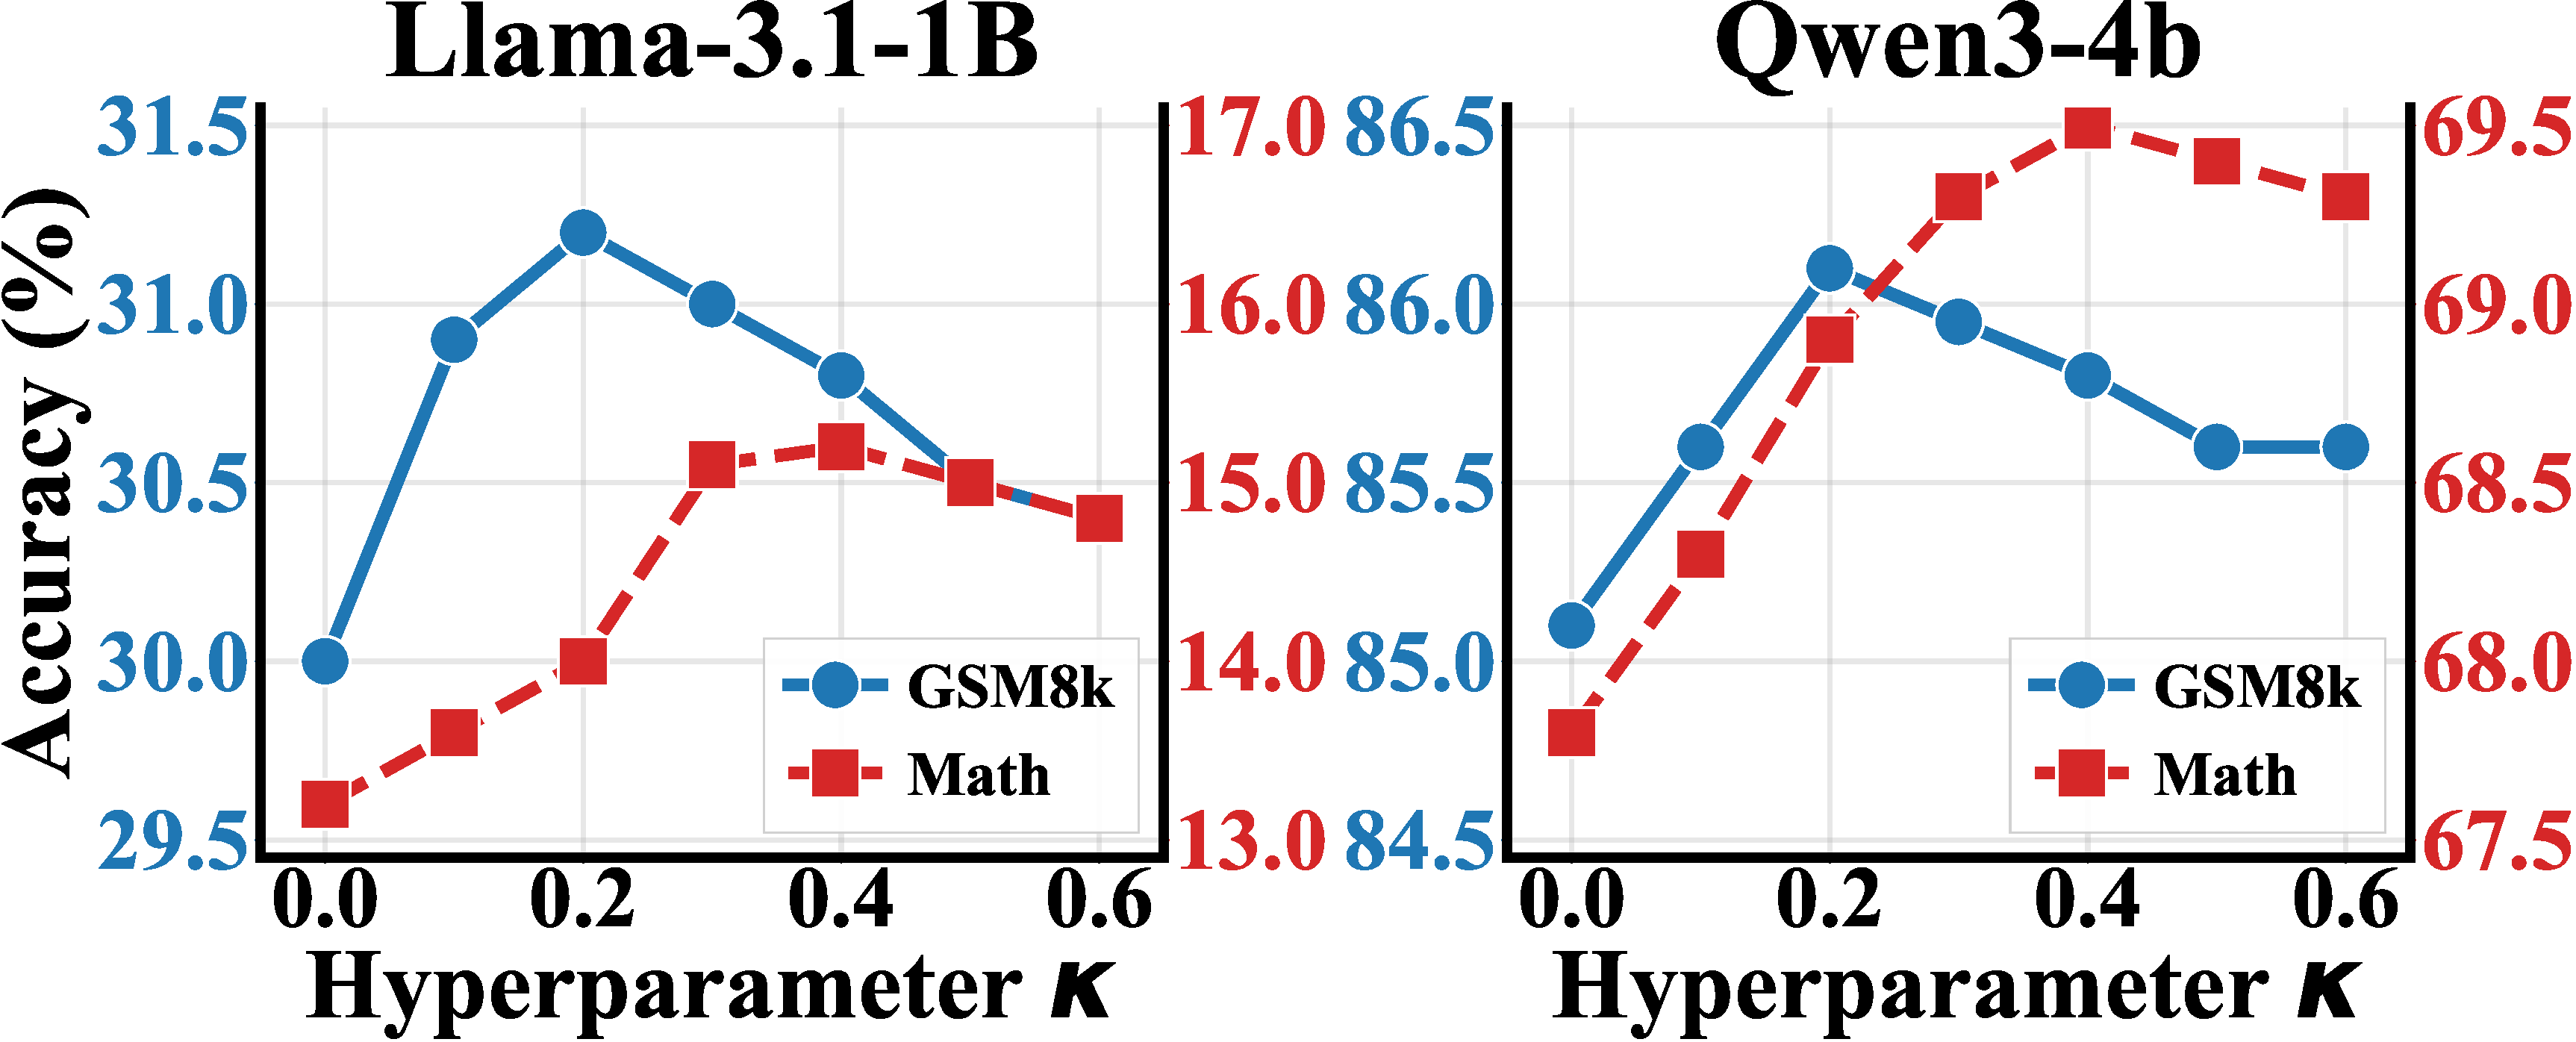
\includegraphics[width=\linewidth]{figs/kappa_analysis.pdf}
    \caption{
     \textbf{Hyperparameter analysis for $\kappa$.} The value $\kappa$ is chosen from $\{0, 0.1, 0.2, 0.3, 0.4, 0.5, 0.6\}$.
     }
    \label{fig: kappa}
\end{figure}

\textbf{Hyperparameter Analysis.}
The token \bk budget $\kappa$ serves as a critical hyperparameter controlling the trade-off between correction capability and generation efficiency. We evaluate the impact of varying $\kappa \in \{0, 0.1, 0.2, 0.3, 0.4, 0.5, 0.6\}$ across two distinct models (Llama-3.2-1B and Qwen3-4B) on both \textsc{Gsm8k} and \textsc{Math} datasets in Figure~\ref{fig: kappa}. 
We observe that the optimal $\kappa$ is highly correlated with task complexity. 
For the simpler \textsc{Gsm8k} benchmark, performance peaks at a lower budget of $\kappa=0.2$. 
Beyond this point, performance slightly degrades, suggesting that excessive budgets on simpler tasks may encourage "over-deliberation", i.e., unnecessary edits that introduce generation noise without improving accuracy.
Conversely, for the more challenging \textsc{Math} dataset, the performance curve shifts rightward, peaking at $\kappa=0.4$. 
This indicates that complex reasoning chains require a larger {correction window} to effectively rectify deep errors. 
Notably, this pattern is consistent across model scales.
Both the 1B and 4B models exhibit the same optimal $\kappa$ values for respective datasets, suggesting that the correction budget is a property of the task's reasoning depth rather than the model capacity.
Based on these empirical findings, we adopt a task-adaptive configuration, setting $\kappa=0.2$ for \textsc{Gsm8k} and $\kappa=0.4$ for \textsc{Math} in our main experiments to maximize the efficiency-accuracy trade-off.

\begin{figure}
    \centering
    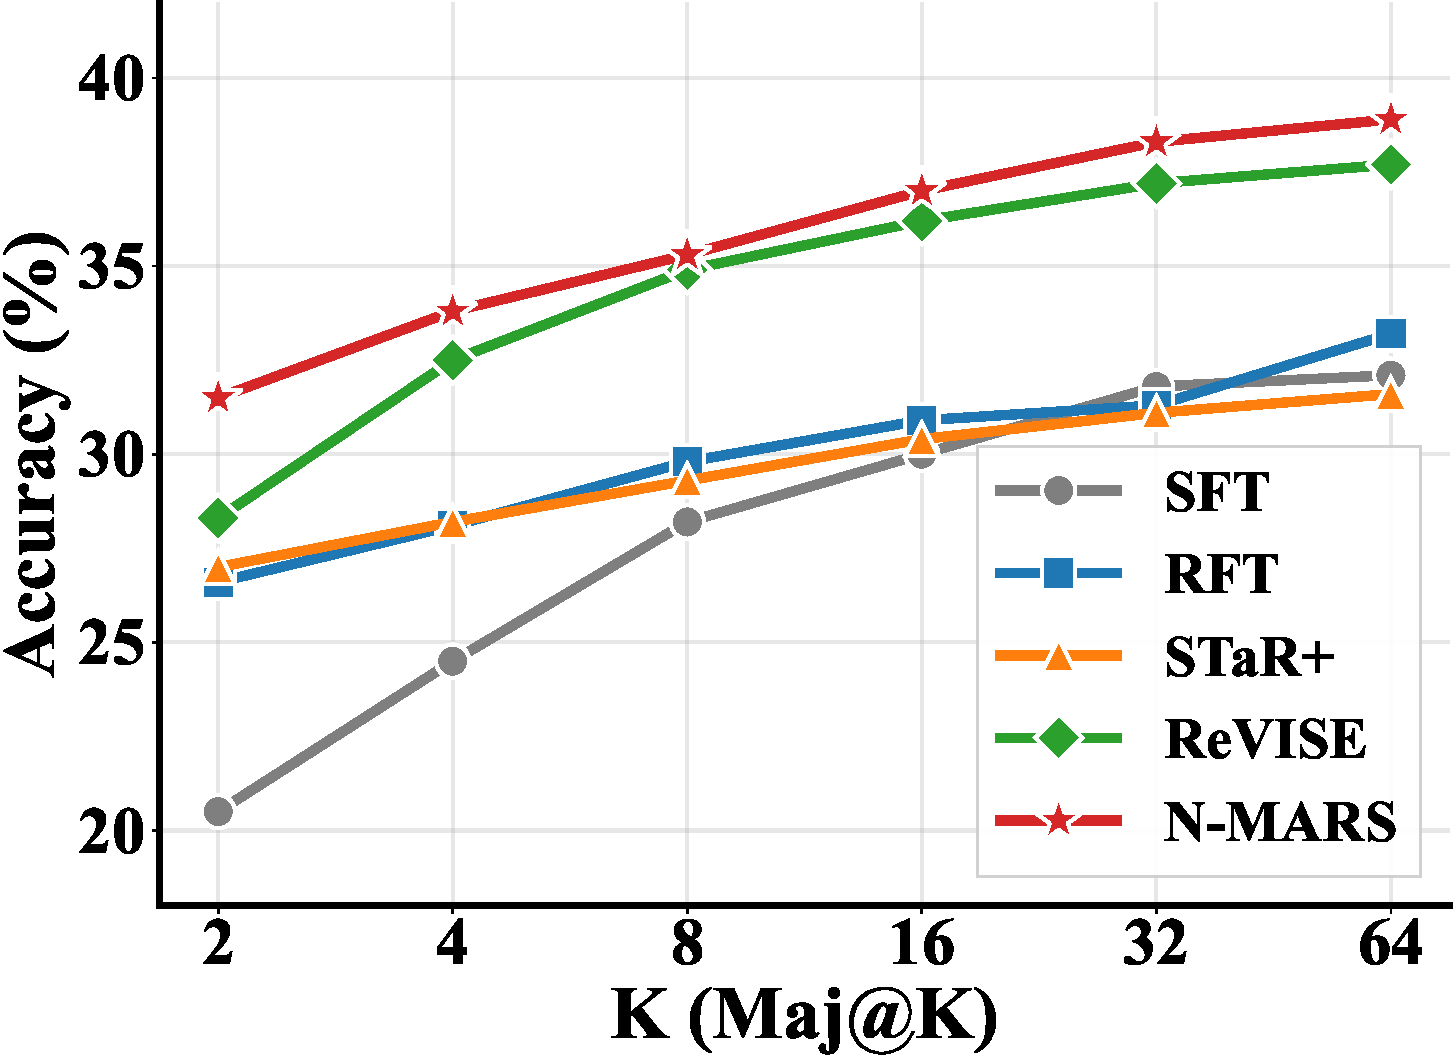
\includegraphics[width=0.95\linewidth]{figs/test_time_scaling.pdf}
    \caption{\textbf{Test-time Scaling Analysis.} Majority voting accuracy (maj@$k$) on \textsc{Gsm8k} with Llama-3.2-1B as the number of samples $k$ increases from 2 to 64.}
    \label{fig: test-time scaling}
\end{figure}
\textbf{Test-time Scaling.}
We evaluate test-time scaling by measuring majority voting accuracy (maj@$k$) as the number of sampled responses increases from 2 to 64 (Figure~\ref{fig: test-time scaling}).
SFT-based methods (SFT, RFT, STaR+) exhibit diminishing returns: RFT improves only $+6.6\%$ and STaR+ only $+4.6\%$ from maj@2 to maj@64, suggesting that these methods converge to a narrow distribution with limited diversity.
In contrast, RL-based methods demonstrate stronger scaling: ReVISE gains $+9.4\%$ across the same range.
\modelname achieves the best scaling behavior, starting from a higher baseline ($31.5\%$ at maj@2 vs.\ $28.3\%$ for ReVISE) and maintaining consistent gains to reach $38.9\%$ at maj@64.
This advantage stems from non-monotonic generation, i.e., the ability to backtrack and explore alternative reasoning paths, which yields a more diverse sample distribution, which majority voting effectively exploits.